\documentclass[10pt]{article}
%----------Packages----------
\usepackage[utf8]{inputenc}
\usepackage[landscape,left=5mm,right=5mm,top=7mm,bottom=7mm]{geometry}
\usepackage{amsmath,amssymb}
\usepackage{multicol}
\usepackage{blindtext}
\usepackage{graphicx}
\usepackage[shortlabels]{enumitem}
%----------Page formatting----------
\pagenumbering{gobble}
\setlength{\parindent}{0pt}
\setlength{\parskip}{2pt}
\renewcommand\labelitemi{$\vcenter{\hbox{\tiny$\bullet$}}$}

%----------Symbols----------
\newcommand{\ep}{\epsilon}

%----------General----------
\newcommand{\ds}{\displaystyle}
\newcommand{\tab}{\hspace{.02\textwidth}}
\newcommand{\inv}{^{-1}}
\newcommand{\twoEqn}[4]{$\makebox[#3][l]{$#1$} \makebox[#4][l]{$#2$}$}
\newcommand{\threeEqn}[6]{$\makebox[#4][l]{$#1$} \makebox[#5][l]{$#2$} \makebox[#6][l]{$#3$}$}

%----------Vectors----------
\newcommand{\norm}[1]{\left|#1\right|}
\newcommand{\vb}[1]{\mathbf{#1}}
\newcommand{\vu}[1]{\vb{\hat{#1}}}

\newcommand{\A}{\vb A}
\newcommand{\B}{\vb B}
\newcommand{\D}{\vb D}
\newcommand{\E}{\vb E}
\newcommand{\F}{\vb F}
\renewcommand{\H}{\vb H}
\newcommand{\I}{\vb I}
\newcommand{\J}{\vb J}
\newcommand{\K}{\vb K}
\newcommand{\N}{\vb N}
\newcommand{\M}{\vb M}
\renewcommand{\P}{\vb P}

\renewcommand{\a}{\vb a}
\renewcommand{\b}{\vb b}
\newcommand{\f}{\vb f}
\renewcommand{\l}{\vb l}
\newcommand{\m}{\vb m}
\newcommand{\p}{\vb p}
\renewcommand{\r}{\vb r}
\renewcommand{\v}{\vb v}

\newcommand{\n}{\vu n}
\newcommand{\rh}{\vu r}
\newcommand{\sh}{\vu s}
\newcommand{\xh}{\vu x}
\newcommand{\yh}{\vu y}
\newcommand{\zh}{\vu z}
\newcommand{\thetahat}{\boldsymbol{\hat{\theta}}}
\newcommand{\phihat}{\boldsymbol{\hat{\phi}}}

%----------Brackets----------
\newcommand{\lrb}[1]{\left(#1\right)}
\newcommand{\sqb}[1]{\left[#1\right]}
\let\originalleft\left
\let\originalright\right
\renewcommand{\left}{\mathopen{}\mathclose\bgroup\originalleft}
\renewcommand{\right}{\aftergroup\egroup\originalright}

%----------Differentiation----------
\renewcommand{\d}{d}
\newcommand{\dv}[2]{\frac{\d #1}{\d #2}}
\newcommand{\ddv}[2]{\frac{\d^2 #1}{\d #2^2}}
\newcommand{\pd}[2]{\frac{\partial #1}{\partial #2}}
\newcommand{\pdd}[2]{\frac{\partial^2 #1}{\partial #2^2}}

%----------Grad, Div, Curl, Laplacian----------
\newcommand{\grad}{\boldsymbol\nabla}
\newcommand{\divg}{\boldsymbol\nabla\cdot}
\newcommand{\curl}{\boldsymbol\nabla\times}
\newcommand{\lap}{\grad^2}

%----------PHYS 301----------
\newcommand{\enc}{\text{enc}}
\newcommand{\en}{\ep_0}
\newcommand{\mn}{\mu_0}
\newcommand{\rsep}{\mbox{$\resizebox{.09in}{.08in}{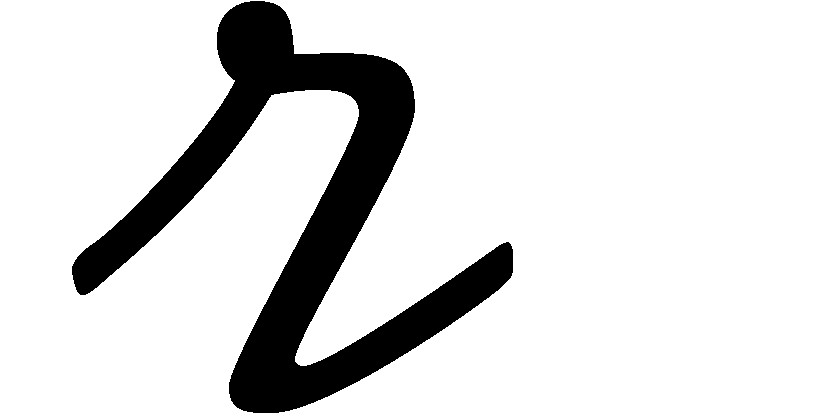
\includegraphics[trim= 1em 0 14em 0,clip]{assets/ScriptR}}$}}
\newcommand{\rsepb}{\mbox{$\resizebox{.09in}{.08in}{
\includegraphics[trim= 1em 0 14em 0,clip]{assets/BoldR}}$}}
\newcommand{\rsepu}{\vu\rsepb}
\newcommand{\cc}{\frac{1}{4\pi\en}} % Coulomb's constant
\renewcommand{\above}{_\text{above}}
\newcommand{\below}{_\text{below}}
\newcommand{\emf}{\mathcal{E}}

%----------Sections----------
\makeatletter
\renewcommand{\section}{\@startsection{section}{1}{0ex}
                                {-2ex}
                                {0.7ex}
                                {\normalfont\large\bfseries}}
\renewcommand{\subsection}{\@startsection{subsection}{2}{0ex}
                                {-0.4ex}
                                {0.4ex}
                                {\normalfont\normalsize\bfseries}}
\makeatother
\setcounter{secnumdepth}{0}

%----------Info----------
\newcommand*{\course}{PHYS 301} 

%----------Document Begins Here----------
\begin{document}

\begin{center}
    \LARGE{\textbf{\course \ Formula Sheet}}
\end{center}

\begin{multicols*}{3}

\section{Maxwell's Equations}

{\renewcommand{\arraystretch}{2}
\begin{tabular}{p{8em}p{12em}}
    $\ds\divg\E=\frac\rho\en$ & $\ds\divg\B=0$ \\
    $\ds\curl\E=-\pd\B t$ & $\ds\curl\B=\mu_0\J+\mn\en\pd\E t$ \\ 
    $\ds\oint\E\cdot\d\a=\frac{Q_\enc}{\en}$ & $\ds\oint\B\cdot\d\a=0$ \\
    $\ds\oint\E\cdot\d\l=-\frac{\d\Phi_B}{\d t}$ & $\ds\oint\B\cdot\d\l=\mu_0 I_\enc+\en\mn\frac{\d\Phi_E}{\d t}$ \\
\end{tabular}}

\section{Electrostatics}

\subsection{Electric Field}

Coulomb's law:

\tab $\ds\F=\cc\frac{qQ}{\rsep^2}\rsepu$

Electric field:

\tab\twoEqn{\ds\F=Q\E}{\E=-\grad V}{10em}{10em}

E-field due to point charges:

\tab $\ds\E(\r)=\cc\sum_{i=1}^n\frac{q_i}{\rsep_i^2}\rsepu_i$

E-field due to continuous charge distribution:

\tab $\ds\E(\r)=\cc\int\frac{\rsepu}{\rsep^2}\d q=\cc\int\frac{\rho(\r')\rsepu}{\rsep^2}\d\tau'$

Gauss's law:

\tab $\ds\oint\E\cdot\d\a=\frac{Q_\enc}{\en}$

\subsection{Electric Potential}

\tab $\ds V(b)-V(a)=-\int_a^b \E\cdot\d\l$

Poisson's equation:

\tab $\lap V=-\rho/\en$

Potential due to continuous charge distribution:

\tab $\ds V(\r)=\cc\int\frac 1\rsep\d q=\cc\int\frac{\rho(\r')}{\rsep}\d\tau'$

\subsection{Work and Energy in Electrostatics}

Energy of point charges:

\tab $\ds W=\frac 12\sum_{i=1}^n q_iV(\r_i)$

Energy of continuous charge distribution:

\tab\twoEqn{\ds W=\frac 12\int\rho V\d\tau}{\ds W=\frac\en 2\int_{\text{all space}} E^2\d\tau}{10em}{10em}

\subsection{Conductors}

Electric field immediately outside a conductor:

\tab $\ds \E=\frac\sigma\en\n$

Surface charge:

\tab $\ds \sigma=-\en\pd Vn$

Capacitors:

\tab\twoEqn{\ds C=\en\frac Ad}{Q=CV}{10em}{10em}

\tab $\ds W=\frac 12CV^2=\frac 12\frac{Q^2}{C}=\frac 12 QV$

\section{Potentials}

Laplace's equation:

\tab $\ds \lap V=\pdd Vx+\pdd Vy+\pdd Vz=0$

\subsection{Separation of Variables}

\tab $\ds\int_0^a\sin\lrb{\frac{n\pi x}{a}}\sin\lrb{\frac{m\pi x}{a}}\d x=\begin{cases}
    0 & \text{if }n\ne m \\
    a/2 & \text{if }n=m
\end{cases}$

Legendre polynomials:

\begin{itemize}[noitemsep,topsep=0pt]
    \item $P_0(x)=1$
    \item $P_1(x)=x$
    \item $P_2(x)=(3x^2-1)/2$
    \item $P_3(x)=(5x^3-3x)/2$
\end{itemize}

Solution to Laplace in spherical ($\phi$ independent):

\tab $\ds V(r,\theta)=\sum_{l=0}^\infty\lrb{A_lr^l+\frac{B_l}{r^{l+1}}}P_l(\cos\theta)$

\subsection{Multipole Expansion}

Axial multipole ($\alpha$ is between $\r$ and $\r'$):

\tab $\ds \cc\sum_{n=0}^\infty\frac{1}{r^{n+1}}\int(r')^nP_n(\cos\alpha)\rho(\r')\d\tau'$

Monopole, Dipole, Quadrupole:

\begin{tabular}{p{13em}p{8em}}
    $\ds V_0(\r)=\cc\frac Qr$ & $\ds Q=\int\rho(\r')\d\tau'$ \\
    $\ds V_1(\r)=\cc\frac{\p\cdot\rh}{r^2}$ & $\ds \p=\int\r'\rho(\r')\d\tau'$ \\
    $\ds V_2(\r)=\cc\sum_{ij}\frac{Q_{ij}\hat r_i\hat r_j}{r^2}$ \\
\end{tabular}

\hspace{0.3em} $\ds Q_{ij}=\int\frac{\rho(\r')}{2}\lrb{3r_i'r_j'-(r')^2\delta_{ij}}\d\tau'$

\section{Electric Fields in Matter}

Dipole torque, force, and energy:

\tab\threeEqn{\N=\p\times\E}{\F=\grad(\p\cdot\E)}{U=-\p\cdot\E}{6.5em}{7.5em}{7em}

Bound charges:

\tab\twoEqn{\sigma_b=\P\cdot\n}{\rho_b=-\divg\P}{10em}{10em}

Electric displacement:

\tab\twoEqn{\D=\en\E+\P}{\ds\oint\D\cdot\d\a=Q_{f,\enc}}{10em}{10em}

\subsection{Linear Dielectrics}

Polarization:

\tab $\ds \P=\en\chi_e\E$

Electric displacement:

\tab $\D=\en(1+\chi_e)\E=\ep\E$

Energy:

\tab $\ds W=\frac 12\int\D\cdot\E\,\d\tau$

\subsection{Boundary Conditions in Electrostatics}

\begin{itemize}[itemsep=0pt,topsep=0pt]
    \item $E\above^\perp-E\below^\perp=\sigma/\en$
    \item $E\above^\parallel=E\below^\parallel$
    \item $V\above=V\below$
    \item $D\above^\perp-D\below^\perp=\sigma_f$
    \item $D\above^\parallel-D\below^\parallel=P\above^\parallel-P\below^\parallel$
\end{itemize}

\section{Magnetostatics}

Lorentz force law:

\tab $\F=q(\E+\v\times\B)$

Currents:

\tab\threeEqn{\I=\lambda\v}{\K=\sigma\v}{\J=\rho\v}{7em}{7em}{7em}

Magnetic force on wire:

\tab $\ds\F_{\text{mag}}=I\int\lrb{\d\l\times\B}$

Continuity equation:

\tab $\ds\divg\J=-\pd\rho t$

Biot-Savart law:

\tab $\ds\B(\r)=\frac{\mn}{4\pi}\int\frac{\I\times\rsepu}{\rsep^2}\d l'=\frac{\mn}{4\pi}\int\frac{\d \l'\times\rsepu}{\rsep^2}$

Ampere's law:

\tab $\ds\oint\B\cdot\d\l=\mn I_\enc$

\newpage
\subsection{Magnetic Vector Potential}

\tab $\B=\curl\A\quad\text{where}\quad\divg\A=0$ 

Vector potential Poisson's equation:

\tab $\lap\A=-\mn\J$

Vector potential when $\J\to\vb 0$ at infinity:

\tab $\ds\A(\r)=\frac{\mn}{4\pi}\int\frac{\J(\r')}{\rsep}\d\tau'$

Multipole expansion of a current loop:

\tab $\ds\A(\r)=\frac{\mn}{4\pi}\sum_{n=0}^\infty\frac{1}{r^{n+1}}\oint(r')^nP_n(\cos\alpha)d\l'$

Magnetic dipole with vector area $\a$:

\tab $\ds\A_{\text{dip}}(\r)=\frac{\mn}{4\pi}\frac{\m\times\rh}{r^2}$

\tab $\ds\m=I\int\d\a=I\a$

\section{Magnetic Fields in Matter}

Dipole torque, force, and energy: 

\tab\threeEqn{\N=\m\times\B}{\F=\grad(\m\cdot\B)}{U=-\m\cdot\B}{6.5em}{7.5em}{7em}

Bound currents:

\tab\twoEqn{\J_B=\curl\M}{\K_B=\M\times\n}{10em}{10em}

Auxiliary field:

\tab\twoEqn{\ds\H=\frac\B\mn-\M}{\ds\oint\H\cdot\d\l=I_{f,\enc}}{10em}{10em}

\subsection{Linear Media}

Magnetization:

\tab $\M=\chi_m\H$

Auxiliary field:

\tab $\B=\mn(\H+\M)=\mn(1+\chi_m)\H=\mu\H$

\subsection{Boundary Conditions in Magnetostatics}

\begin{itemize}[itemsep=0pt,topsep=0pt]
    \item $B\above^\parallel-B\below^\parallel=\mn K$
    \item $B\above^\perp=B\below^\perp$
    \item $\A\above=\A\below$
    \item $H\above^\perp-H\below^\perp=-(M\above^\perp-M\below^\perp)$
    \item $H\above^\parallel-H\below^\parallel=\K_f\times\n$
\end{itemize}

\section{Miscellaneous Formulas}

Electric field of dipole:

\tab $\ds\E_{\text{dip}}(r,\theta)=\frac{\p}{4\pi\en r^3}\lrb{2\cos\theta\,\rh+\sin\theta\,\thetahat}$

\newcolumn
\section{Electrodynamics}

Force per unit charge:

\tab $\f=\v\times\B$

Electromotive force:

\tab\twoEqn{\ds\emf=\oint\f\cdot\d\l}{\emf=vBh}{10em}{10em}

Flux rule:

\tab $\ds\emf=-\dv\Phi t$

\section{Vector Derivatives}

\subsection{Cartesian}

Gradient:

\tab $\ds\grad f=\pd fx\xh+\pd fy\yh+\pd fz\zh$

Divergence:

\tab $\ds\divg\v=\pd{v_x}{x}+\pd{v_y}{y}+\pd{v_z}{z}$

Curl:

{\small$\ds\curl\v=\lrb{\pd{v_z}{y}-\pd{v_y}{z}}\xh+\lrb{\pd{v_x}{z}-\pd{v_z}{x}}\yh+\lrb{\pd{v_y}{x}-\pd{v_x}{y}}\zh$}

\subsection{Spherical}

Gradient:

\tab $\ds\grad f=\pd fr\rh+\frac 1r\pd f\theta\thetahat+\frac{1}{r\sin\theta}\pd f\phi\phihat$

Divergence:

\tab $\ds\divg\v=\frac{1}{r^2}\pd{}{r}\lrb{r^2v_r}+\frac{1}{r\sin\theta}\pd{}{\theta}(\sin\theta v_\theta)+\frac{1}{r\sin\theta}\pd{v_\phi}{\phi}$

Curl:

\tab $\ds\curl\v=\frac{1}{r\sin\theta}\sqb{\pd{}{\theta}\lrb{\sin\theta v_\phi}-\pd{v_\theta}{\phi}}\rh$

\tab $\ds+\frac 1r\sqb{\frac{1}{\sin\theta}\pd{v_r}{\phi}-\pd{}{r}(rv_\phi)}\thetahat
+\frac 1r\sqb{\pd{}{r}(rv_\theta)-\pd{v_r}{\theta}}\phihat$  

\subsection{Cylindrical}

Gradient:

\tab $\ds\grad f=\pd fs\sh+\frac 1s\pd f\phi\phihat+\pd fz\zh$

Divergence:

\tab $\ds\divg\v=\frac 1s\pd{}{s}(sv_s)+\frac 1s\pd{v_\phi}{\phi}+\pd{v_z}{z}$

Curl:

\tab $\ds\curl\v=\sqb{\frac 1s\pd{v_z}{\phi}-\pd{v_\phi}{z}}\sh$

\tab $\ds+\sqb{\pd{v_s}{z}-\pd{v_z}{s}}\phihat+\frac 1s\sqb{\pd{}{s}(sv_\phi)-\pd{v_s}{\phi}}\zh$

\section{Fundamental Theorems}

Gradient theorem:

\tab $\ds\int_\a^\b\lrb{\grad f}\cdot\d\l=f(\b)-f(\a)$

Divergence theorem:

\tab $\ds\int\lrb{\divg A}\d\tau=\oint\A\cdot\d\a$

Stoke's theorem:

\tab $\ds\int\lrb{\curl A}\cdot\d\a=\oint\A\cdot\d\l$

\section{Spherical Coordinates}

\tab 
$\begin{cases}
    x=r\sin\theta\cos\phi \\ 
    y=r\sin\theta\sin\phi \\
    z=r\cos\theta
\end{cases}$

\tab
$\begin{cases}
    \xh=\sin\theta\cos\phi\,\rh+\cos\theta\cos\phi\,\thetahat-\sin\phi\,\phihat \\
    \yh=\sin\theta\sin\phi\,\rh+\cos\theta\sin\phi\,\thetahat+\cos\phi\,\phihat \\
    \zh=\cos\theta\,\rh-\sin\theta\,\thetahat
\end{cases}$

\tab
$\begin{cases}
    r=\sqrt{x^2+y^2+z^2} \\
    \theta=\tan\inv\lrb{\sqrt{x^2+y^2}/z} \\
    \phi=\tan\inv(y/x)
\end{cases}$

\tab
$\begin{cases}
    \rh=\sin\theta\cos\phi\,\xh+\sin\theta\sin\phi\,\yh+\cos\theta\,\zh \\
    \thetahat=\cos\theta\cos\phi\,\xh+\cos\theta\sin\phi\,\yh-\sin\theta\,\zh \\
    \phihat=-\sin\phi\,\xh+\cos\phi\,\yh
\end{cases}$

\section{Cylindrical Coordinates}

\tab 
$\begin{cases}
    x=s\cos\phi \\
    y=s\sin\phi \\
    z= z
\end{cases}$

\tab 
$\begin{cases}
    \xh=\cos\phi\,\sh-\sin\phi\,\phihat \\
    \yh=\sin\phi\,\sh+\cos\phi\,\phihat \\
    \zh=\zh
\end{cases}$

\tab 
$\begin{cases}
    s=\sqrt{x^2+y^2} \\
    \phi=\tan\inv(y/x) \\
    z=z
\end{cases}$

\tab 
$\begin{cases}
    \sh=\cos\phi\,\xh+\sin\phi\,\yh \\
    \phihat=-\sin\phi\,\xh+\cos\phi\,\yh \\
    \zh=\zh
\end{cases}$

\rule{\linewidth}{0.1pt}

\scriptsize 
Last updated \today

\end{multicols*}


\end{document}